% File: tex/introduction.tex
% Author: Timo L. R. Halbesma <timo.halbesma@student.uva.nl>
% Version: 0.01 (Initial)
% Date created: Sat Oct 24, 2015 12:28 am
% Last modified: Mon Sep 05, 2016 07:25 PM
%
% Description: Masterthesis, Introduction


\documentclass[MScProj_TLRH_ClusterEnergy.tex]{subfiles}

\begin{document}
\chapter{Introduction}
\label{sec:introduction}

\section{Cosmology: Large-Scale Structure Formation}
\label{sec:structure}

We start with an overview of structure formation in a cosmological context to 
understand why clusters of galaxies of galaxies emit X-ray emission and why
clusters of galaxies are expected to merge with other clusters. Cosmology is the 
study of the universe as a whole, a field based on the fundamental assumptions 
that the universe is isotropic and homogeneous on the largest scales. The current 
cosmological paradigm is the Lambda Cold Dark Matter ($\Lambda$CDM) Big Bang 
model. This framework emerged from numerous observations at different times on 
the cosmological timeline, or epochs, that contribute to a consistent model 
of the universe. The most important observations are the cosmic microwave 
background radiation (CMBR), the Hubble law, type Ia supernova as a function of
redshift $z$, rotation curves of galaxies and the observation of the bullet cluster,
large all-sky surveys of galaxies combined with numerical simulations, and Lyman
$\alpha$ line emission in quasars. The concordance of these observations show 
that energy-matter in the universe is split up in roughly seventy per cent dark 
energy, about twenty-six per cent dark matter, and approximately four per cent 
baryonic matter. All observed electromagnetic radiation originates from the latter.


\subsection*{Cosmic Microwave Background Radiation and the Big Bang}
\label{sec:bigbang}

The universe is thought to have formed in a single event called the Big Bang.
Shortly thereafter, when the age of the universe was \mytilde $10^{-35}$ seconds, 
the small volume of space-time is thought to have undergone a period of rapid 
expansion called inflation. This concept that is critical to concordance cosmology
and fundamentally explains the origin of large-scale structure in the universe. 
During inflation, quantum fluctuations in the inflaton field increased to 
macroscopic proportions as the universe expanded, which caused in ripples in the energy
density of the universe \citep{1981PhRvD..23..347G}. As the universe expanded, 
adiabatic cooling lowered the temperature of the universe reaching the threshold
for nucleosynthesis. The light elements present in the universe have formed in
this era that lasted from around ten seconds to twenty minutes after the big bang.
The state of the universe thereafter can be thought of as a hot primordial soup of free
protons, electrons and photons. The plasma is opaque to electromagnetic radiation:
photons cannot escape as a result of frequent Thomson scattering on the abundantly 
available free electrons and the soup remains ionised. At a certain point in 
time the temperature in the universe reaches the recombination temperature of neutral
hydrogen, roughly $3000$~K, and the free electrons and protons
become bound. The sudden drop in free electrons available for scattering allows 
the photons to escape. This event is called the epoch of recombination 
\citep{1968ApJ...153....1P, 1969JETP...28..146Z, 2000ApJS..128..407S}.
The last time the photons interacted with matter is called the surface of last 
scattering and blackbody radiation from these photons can be observed at present.
Recombination happened around $z$ \mytilde $1100$, thus, the photons are redshifted
to microwave wavelengths. These photons were first observed in 1964 - but published
a year later - by \citet{1965ApJ...142..419P}. This feature, the Cosmic Microwave
Background Radiation (CMBR, Figure~\ref{fig:CMBR}), shows tiny temperature fluctuations of 
a few hundred $\mu$K. The earliest ripples in the cosmic energy density that arose
as a result of the inflated quantum fluctuations have translated into small density
perturbations to the tightly coupled photon-baryon plasma \citep{1970ApJ...162..815P} 
which, in turn, resulted in the small temperature variations observed in the CMBR.

\begin{figure}
\centering
\includegraphics[width=0.78\textwidth]{introduction/cosmology/commander_highres_nogrid.jpg}
\caption{\satellite{Planck} all-sky map showing the universe at the largest scales 
         is isotropic and homogeneous apart from tiny temperature fluctuations of order
         $100 \mu$K. These temperature fluctuations are interpreted as the seeds
         all large-scale structure currently observed has grown from.
         Figure adopted from the \citet{2015arXiv150201582P}.}
         \label{fig:CMBR}
\end{figure}

\subsection*{Cosmological Redshift and Hubble's Law}
\label{sec:redshift}

Big Bang Theory states that ``our whole universe was in a hot dense state, then 
nearly fourteen billion years ago expansion started, wait..." \citep{BigBangTheory}.
Naturally, this requires an expanding universe. An important concept is 
cosmological is redshift, defined as
\begin{align}
    z &= \frac{\lambda_{\text{obs}} - \lambda_{\text{em}}}{\lambda_{\text{obs}}} \quad ,
\end{align}
\noindent where redshift is an increase in the observed wavelength 
$\lambda_{\text{obs}}$ with respect to the emitted wavelength $\lambda_{\text{em}}$.
Conversely, a decrease is called blueshift. Extragalactic sources are redshifted\footnote{
with the exception of the Andromeda galaxy because it is gravitationally bound}, 
classically interpreted as a Doppler shift that relates (low) redshifts to a 
velocity~$v$ via $z\approx v/c$. Redshifted wavelengths correspond to a positive
velocity, indicating that objects are moving away from the observer at Earth.
This collective movement is interpreted as evidence that space-time itself is 
indeed expanding which stretches the wavelength of emitted light, or causes 
the source of emission to move away from us at velocity $v$.

\citet{1929PNAS...15..168H} is the first to observe a linear correlation between
the systematic increase in redshift of `extragalactic nebulae' and the distance 
to these objects. A specific type of stars are Cepheids, variable stars bright
enough to be visible in galaxies other than our own. Moreover, these giants show
a strong correlation between the intrinsic luminosity and the pulsation period. 
A measurement of the period and the observed luminosity, thus, effectively is a 
measure of distance. This method, calibrated on galactic Cepheids using the 
parallax method, can therefore be used to measure the distance to the host galaxy 
of Cepheids. The linear relation between redshift and distance $D$ found is
\begin{align}
    v &= cz = H_0 D \quad ,
\end{align}
\noindent where the Hubble constant $H_0$ with units km/s/Mpc is an important 
cosmological parameter that quantifies the rate of expansion. This observation, 
the Hubble law, does not depend on direction and shows that the universe is
undergoing an isotropic expansion. 

\subsection*{Type Ia Supernovae and Dark Energy}
\label{sec:darkenergy}

Observations show that he rate of expansion increases. Type Ia supernova 
explosions allow for distance measurements beyond $z=1$. White dwarfs in binary
stars can accrete matter until the Chandrasekhar mass is reached. At this point,
a runaway process leads to the explosion of this fixed mass, thus, a fixed energy
is released. Therefore the intrinsic luminosity is known and the distance can be
inferred from the observed luminosity. The redshift can be measured if the host
galaxy of the supernova is known. Surprisingly, supernovae at $z>0.5$ are fainter
\citep{1998AJ....116.1009R, 1999ApJ...517..565P} than expected for sources at a
distance obtained by linear extrapolation of Hubble's law. This observation can
be explained if the universe is expanding at an accelerated rate, which requires
mass-energy in the universe that acts as the opposite of gravity. The first law
of thermodynamics requires a negative pressure in an adiabatically expanding 
vacuum. This naturally places the required reverse-signed gravity in the universe
as having space-time itself costs energy. In this scenario dark energy is the
cosmological constant $\Lambda$, first introduced by Einstein, and this is the
only mathematical quantity in Friedmann cosmology that causes accelerated expansion
of the universe. Details of dark energy are beyond the scope of this thesis, but
we assume that dark energy contributes to seventy per cent of the energy budget
as inferred from type Ia supernovae.

\subsection*{Galaxy Rotation Curves, Bullet Cluster and Dark Matter}
\label{sec:darkmatter}

We now turn to the matter budget of the universe. The majority of matter is
only detected by the gravitational effect it has, whereas all the matter
that emits electromagnetic radiation contributes only to a small part of the 
total gravitating mass. This extra gravitating mass is assumed to originate
from hypothesised weakly interacting particles. 
\newpage
\begin{figure}[ht]
  \centering
  \captionsetup[subfigure]{oneside,margin={-0.25cm,0cm},width=\textwidth}
  \begin{subfigure}[b]{.5\textwidth}
    \centering
    \includegraphics[width=\textwidth]{introduction/cosmology/Andromeda_RotationCurve.png}
    \caption{Rotation curve of the Andromeda galaxy showing that the orbital 
             velocities of stars at large radii flattens out instead of decreases
             as $1/r^2$. Figure adopted from \citet{1970ApJ...159..379R}.}
    \label{fig:andromeda}
  \end{subfigure}%
  ~
  \captionsetup[subfigure]{oneside,margin={0.25cm,0cm}}
  \begin{subfigure}[b]{.5\textwidth}
    \centering
    \includegraphics[width=\linewidth]{introduction/cosmology/1e_xrayimg_lens_sm7.pdf}
    \caption{Bullet shaped gas in a cluster-cluster merger with weak lensing 
             contours overlay shows the gas lags behind the dark matter.
             Figure adopted from \citet{2004ApJ...606..819M}.}
    \label{fig:bullet}
    \end{subfigure}
    \caption{Observations considered compelling evidence for the existence of 
             dark matter.}
    \label{fig:dmproof}
\end{figure}

\noindent This form of matter is believed
to have a significantly lower cross section for electromagnetic interactions 
which results in a lack of electromagnetic radiation. As no light is emitted,
this form of matter is called dark matter. The concept makes its first 
stage-appearance after \citet{1933AcHPh...6..110Z} inferred a significantly 
higher total gravitating mass in the Coma cluster from virial theorem than 
expected based on the luminosity of all stars in the cluster. The dark matter
hypothesis, however, was only accepted by the community decades later when 
observations of the Andromeda galaxy by \citet{1970ApJ...159..379R} showed that
the orbital velocity flattens from a certain radius (Figure~\ref{fig:andromeda}).
Kepler's harmonic law, on the other hand, dictates an orbital velocity of stars
in galaxies inversely proportional the distance of the star to the center of
mass squared. This observation is interpreted as strong evidence in favour of
the existence of dark matter, but perhaps the most compelling is the merging
Bullet cluster (Figure~\ref{fig:bullet}). The galaxy distribution is expected
to follow the potential set by the total mass in the cluster. Furthermore, the
collisional cross section for the individual stars and galaxies is low, thus,
they are not expected to collide. Optical images of clusters show, as expected,
that galaxy mergers are rare events. The hot plasma observed in X-rays, on the
other hand, shows clear signs of interplay. The velocity of the ICM decreases
trough friction while the gas simultaneously heats up. The dark matter 
distribution can be traced using weak and strong gravitational lensing, and 
indeed, the dark matter does not appear to feel the gas pressure. In fact, the
baryonic gas seems to lag behind the dark halo \citep{2004ApJ...606..819M}.
At cosmological scales, the dominant longe-range force-term is gravity. As 
gravity results from mass, gravity is dominated by the ubiquitous dark matter.


\subsection*{Large-scale Galaxy Redshift Surveys and Hierarchical Clustering}
\label{sec:hierarchicalclustering}

The small fluctuations of the cosmic energy density observed in the CMBR have 
grown over time to larger structures ranging from the stars we observe when 
gazing at the night sky, to a rich morphology of galaxies and clusters of galaxies 
on larger scales. This growth of structure is driven by gravitational attractions
that ultimately push the self-gravitating mass to a point where gas pressure can
no longer counter the attractive forces and the system collapses trough the Jeans
instability. This process occurs when the length scale exceeds the Jeans length.
As expansion of the universe decreases the Jeans length, larger structures become 
gravitationally unstable and collapse. The largest modes that have collapse at 
present are clusters of galaxies. The resulting large-scale morphology of matter
in the universe (Figure~\ref{fig:cosmicweb}) is coined `Cosmic web' 
\citep{1996Natur.380..603B}.  This name originates from the observation of a clumpy
filamentary structure that is reminiscent of a rather chaotic spider web. This 
structure is clearly visible in large all-sky galaxy surveys like the Sloan Digital
Sky Survey \citep[SDSS;][]{2000AJ....120.1579Y}, the 2-degree Field Galaxy Redshift
Survey \citep[2dFGRS;][]{2001MNRAS.328.1039C}, and the galaxy redshift survey of the 
Center for Astrophysics \citep[CfA;][]{1989Sci...246..897G}. Interestingly, 
remarkably similar morphologies are found (Figure~\ref{fig:cosmicweb}) when 
plugging the  cosmological parameters inferred from CMBR observations in numerical
$\Lambda$CDM cosmological simulations such as the Milennium Simuation
\citep{2005Natur.435..629S}. The backbone of the sheets of structure is the dark
matter that dominates the potential well. As the dark matter does not feel 
pressure it forms potential wells. The baryonic matter follows behind the dark
and falls towards the bottom of the well, condenses and cools to form the stars, 
galaxies and clusters of galaxies. This explains why these observations reveal
that clusters of galaxies are typically found at junctions of the cosmic filament.
As the baryonic matter is displaced along the cosmic filament, clusters of galaxies are
also expected to interact with one another in highly energetic merger events. This 
allows smaller structures in the universe to further grow hierarchically trough 
these mergers in a bottom-up fashion \citep{1974ApJ...187..425P} and results in 
quasi-spherical clusters. Mergers of clusters are the most energetic events in
the universe since the big bang with a typical kinetic energy of order $10$\Sup{63-64}
erg, and such major mergers are likely to occur several times during the cluster 
lifetime with a rate of once every $2-4$ Gyr \citep{1990MNRAS.245..559E, 1992MNRAS.258..177E}. 

\begin{figure}
\centering
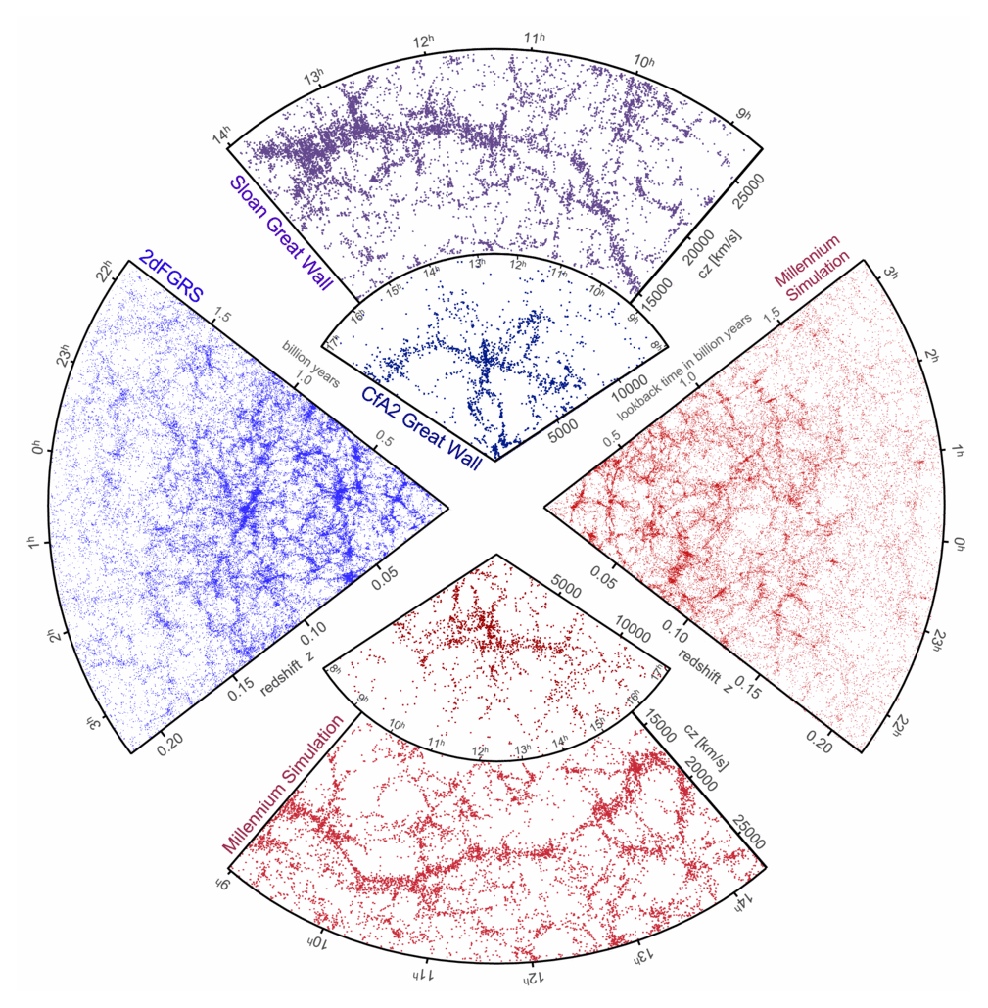
\includegraphics[width=0.6\textwidth]{introduction/cosmology/MilenniumSimuation_SDSS_2fDS.eps}
\caption{The Cosmic Web seen in all-sky redshift serveys (CfA, SDSS, 2dFGRS).
         Cosmological simulations recreate this geometry and the observed
         magnitudes. Image adopted from \citet{2006Natur.440.1137S}.}
\label{fig:cosmicweb}
\end{figure}

\subsection*{Clusters of Galaxies and Baryonic Matter}
\label{sec:clusterbaryons}

Current observations comprise a few dozen well-known, well-studied clusters of
galaxies. Perhaps the best-known examples are the Virgo, Coma and Bullet cluster,
while the Cygnus cluster is relatively unknown as a cluster of galaxies.
Clusters are made up of several tens to thousands of optically visible 
galaxies that, together with the hot intra cluster gas further discussed in 
section~\ref{sec:clustergas}, reside in the dark matter dominated potential
well. We further address the shape of the dark matter halo in 
section~\ref{sec:darkmatter}. Clusters of galaxies are the
largest virialised structures in the universe with typical sizes (diameter) in 
the order of a few megaparsec (1 parsec = 3.09$\cdot$10\Sup{16} m) and typical 
masses of 10\Sup{14-15} M\Sun (1 solar mass = 1.9889$\cdot$10\Sup{30} kg). All
visible baryonic matter locked up in the stars and galaxies contributes to 
\mytilde ten per cent of the baryonic mass in clusters of galaxies while the 
majority of the baryonic matter is found in intra cluster medium (ICM). As stated
earlier, the dark matter component plays a major role in clusters of galaxies as
it dominates the gravitational potential because dark matter contributes to roughly
ninety per cent of the total mass in clusters. The ICM is heated to 
temperatures of order 10\Sup{7-8}~K, or typical kT in the range \mytilde~2-15~keV 
\citep{2007ARA&A..45..117M}. These energies are
well within the detection range of X-ray satellites. As the distribution of the
hot gas follows the shape of the potential, clusters are ideal testbeds to study 
the distribution of dark matter in the universe. Moreover, the same potential sets
the galaxy distribution and the velocity dispersion along the line of sight of 
the optically visible galaxies in the cluster. This allows to cross-check results
inferred both from optical and from X-ray observations to develop self-consistent 
models of clusters of galaxies. This makes clusters of galaxies ideal to 
test and constrain cosmological models.


\subsection*{Evolution of the Universe}
\label{sec:evolution}

The cosmological model in combination with the cosmological parameters allows
astronomers to predict the ultimate faith of the universe. The evolution of the 
universe depends strongly on the density parameter $\Omega_{\text{tot}}= 
\Omega_M + \Omega_r + \Omega_\Lambda$. The first parameter, the mass density, is 
the sum of the baryonic and dark matter, the second being the radiation denisty, 
while the latter constitutes the contribution of the cosmological constant 
$\Lambda$ that results in a positive vacuum energy density, thus a negative pressure
that results in accelerated expansion of the universe. The mass density can be 
expressed as the ratio of the true mass density of the universe $\rho_m$ over the 
critical density

\begin{align}
    \rho_{\text{crit}} &= \frac{3H(z)^2}{8\pi G} \label{eq:rhocrit} \quad ,
\end{align}

\noindent where $H$ is the Hubble constant as a function of redshift $z$.
The $\Omega_{\text{tot}} > 1$ case, which is when the universe is `closed',
will ultimately result in a collapse of the universe commonly referred to as the
Big Crunch, while the universe is thought of as `open' for $\Omega_{\text{tot}} < 1$
because spacetime undergoes continuous monotonic expansion ad infinitum. For unity 
the universe is called `flat' and the expansion rate will decline exponentially.
Clusters of galaxies provide excellent observational constrains on the mass density 
parameter. The numerical value can be inferred from observations of the mass 
distribution, the number density of clusters, and the amount of substructure within 
clusters of galaxies. Clusters of galaxies can thus be used to probe the evolution
of the universe as a whole.

These observations combined with evidence gathered from different epochs on the
cosmological timeline has lead to convincing support for the $\Lambda$CDM model.
In particular, understanding of the CMBR has contributed greatly to constrain 
values of the cosmological parameters. For example, the numerical values are found in 
the Wilkinson Microwave Anisotropy Probe (\satellite{WMAP}) nine year data release
that features the final maps and results \citep{2013ApJS..208...20B}. The 
\satellite{Planck} spacecraft is currenly in orbit and is expected to further
improve these measurements \citep{2015arXiv150201582P}. Our current best understanding 
of the observations has lead to the believe that the universe is flat as the the 
measured total density $\Omega_{\text{tot}} \approx 1$ with the dominant 
contribution arising from the vacuum energy density. The typical values, or a generic
set of cosmoligical parameters if you will, assumes a Hubble parameter 
$H_0 = 70$ km/s/Mpc, $\Omega_{M,0} = 0.3$, $\Omega_{\Lambda,0} = 0.7$. Note that
the following quantities scale with the reduced Hubble parameter 
$h=H_0 / (100$~km/s/Mpc$)$. The X-ray luminosity scales as $L_x \propto h^{-2}$,
the core radius (see equation~\eqref{eq:betamodel}) as $r_c \propto h^{-1}$, and the
mass of the intra cluster gas as $M_g\propto (L_x r_c^3)^{1/2} = h^{-5/2}$.






\section*{Cosmological Calculator}

The main use of cosmology for astronomers is that it allows to convert an angle 
on the sky of an object at given redshift $z$ to a physical distance in kpc.
\citet{2006PASP..118.1711W} provides an online cosmological converter that
implements the theoretical considerations and allows to input a given set of
cosmological parameters and a redshift. This tool has been ported to \code{Python} 
by \citet{CosmologyCalculator}. We shamelessly copy-pasted the latter. The 
cosmological calculator assumes a radiation density that results from blackbody 
radiation with temperature $T_0 = 2.72528$~K (CMBR) plus three massless neutrino
species. The comoving distance divided by the Hubble radius $H_0/c$ is denoted 
as $Z$ given by

\begin{align}
    Z &= \int\limits_{1/(1+z)}^{1} \frac{\mathrm{d}a}{a} 
    \left( \frac{\Omega_m}{a} + \frac{\Omega_r}{a^2} 
+ \Omega_{\Lambda}a^2 + (1-\Omega_{\text{tot}}) \right)^{-1/2} \\
\intertext{where $a$ is the cosmological scale factor normalised at $a=1$ in the current
epoch. Here $\mathrm{d}a/a$ can also be written as $\mathrm{d}z/(1+z)$ while integrating from 
$0$ to $z$. Defining}
J(x) &= \begin{cases}
            \sin\left(\sqrt{-x}\right)/\sqrt{-x} & \text{for} \, x<0 \\
            \sinh \left(\sqrt{x}\right)/\sqrt{x} & \text{for} \, x > 0\\
            1 + x/6 + x^2/120 + ... + x^n/(2n+1)! & \text{for} \, x \approx 0
        \end{cases}\\
\intertext{where the three different cases represent an open, closed and flat universe.
           This gives the formula to convert from seconds of arc to kilo parsec
           in a flat universe as}
        1 \, \text{arcsec} &= \frac{1}{1+z} \, \frac{cZ}{H_0} \,
           J\left(\sqrt{|(1-\Omega_{\text{tot}}|} Z^2\right) 
           \frac{360}{2 \pi} \, 3600 \, \frac{1}{1000} \, \text{kpc} \label{eq:arcsec2kpc}
\end{align}

Here $cZ/H_0$ is needed to convert back to physical units in Mpc from per unit
Hubble radius, $360/(2\pi)$ converts the angle in radians to degrees, $3600$ from
degrees to arcseconds, and finally we divide by $1000$ to convert from Mpc to kpc.

Cygnus~A has a redshift of $z=0.0562$ \citep{1997ApJ...488L..15O}, at which
one conveniently finds that $1$" approximately corresponds to $1$ kpc. More 
precise, $1$" \mytilde \, $1.091$ using the typical cosmological parameters. \\
%eq.~\eqref{eq:arcsec2kpc}



\section{Structure of Dark Matter Haloes}
\label{sec:darkmatter}

The NFW profile is widely accepted to describe the distribution of dark matter.
\citet{1996ApJ...462..563N} show that this profile spans over two orders of 
magnitude in radius, and is valid for a wide range of masses starting at small 
dwarf galaxies ($10^{12}$ M\Sun) all the way up to the most massive ($10^{15}$
M\Sun) clusters of galaxies. Furthermore, a seemingly inconsistent picture of 
typical values for the dark matter core radii is solved by the NFW profile. 
Specifically, arcs observed in gravitational lensing studies show typical core 
radii of $20-60$~kpc \citep{1988ApJ...324L..37G}, while X-ray observations show 
typical values in the range $100-200$~kpc \citep{1991A&ARv...2..191F}. This 
inconsistency is solved naturally when using the NFW-profile. This seminal work 
provides the basis for any model that includes dark matter, specifically when 
numerical simulations on the scale of galaxies or clusters of galaxies are in play.
The NFW-profile is defined as

\begin{align}
    \rho(r) &\propto \frac{1}{r \left( 1 + \frac{r}{r_s} \right)^2}
        \label{eq:nfw} \quad ,
\end{align}

\noindent where $r_s = r_{200}/c_{NFW}$ is the scaling radius and $c_{NFW}$
is the concentration parameter. Note that contrary to the core
radius $r_c$ in the beta-model such that for $r<r_c$ the density
is roughly constant, the scale radius is the radius over which
the profile changes shape. The physical meaning of the scale radius is
that near this radius the profile is roughly isothermal. 

\citet{1990ApJ...356..359H} provides an elegant equation similar to the
NFW-profile but resulting in analytical solutions when integrated. This formula 
was originally derived as an analytical alternative for the de Vaucouleurs $R^{1/4}$
profile for elliptical galaxies. 

\begin{align}
    \rho(r) &= \frac{M}{2 \pi} \frac{a}{r(r+a)^3} \label{eq:hernquist} \\
    M_{DM}(<r) &= M \frac{r^2}{(r+a)^2} \label{eq:hernquist_mass} \\
    \phi(r) &= - \frac{GM}{r+a} \label{eq:hernquist_gravpot} \\
    \psi(r) &= - \left( \frac{a}{GM} \right) \cdot \phi(r) = \frac{a}{a+r} \label{eq:hernquist_psi} \quad ,
\end{align}

The quantity $a$ is a scale length. The mass profile is obtained by integrating
the density profile over spherical shells of volume, $\mathrm{d}V = 4 \pi r^2 
\mathrm{d}r$, from $0$ to $r$ and leads to an analytical expression. Note that the
quantity $M$ in the mass profile corresponds to a total, finite mass and would 
be the equivalent of integrating the density profile from $0$ to $\infty$. In 
this sense, the Hernquist profile has a finite total matter mass: the mass profile 
converges towards to $M$ as $r\rightarrow \infty$. The potential $\phi(r)$ follows
by integrating the Poison equation. Dividing out the constants yields a very
powerful form, the dimensionless potential $\psi(r)$ that spans a range from 
$0 (r\rightarrow \infty)$ to $1 (r\rightarrow 0).$ Moreover, the distribution 
function, density of states, projected X-ray surface brightness and the velocity
dispersion are all described by elementary functions. Owing to the similarities
between the NFW-profile and the de Vaucouleurs $R^{1/4}$ profile, the Hernquist 
profile is also an accurate alternative for the NFW-profile to describe dark matter
haloes, simply by replacing the total mass $M$ by the total dark matter mass 
$M_{\text{DM}}$. This analytical expression is first implemented in a numerical
routine by \cite{2005MNRAS.361..776S} to study the effects of feedback from stars
and black holes in galaxy mergers. The authors note that the inner shape of the
profile is equal to the NFW-profile while the faster decline in the outer part
results in a converging mass profile. This can clearly be seen in 
Figure~\ref{fig:Hernquist_NFW_equal}. As stated earlier, the NFW-profile holds 
for masses ranging from dwarf galaxies to the richest clusters of galaxies. This 
implies that the Hernquist profile is also a viable solution for numerical 
simulations of clusters of galaxies.

To force consistency between the NFW-profile and the Hernquist profile
(such that $\rho_{\text{DM}} = \rho_{NFW}$ for $r<<r_{200}$), the hernquist 
scale length is set by the concentration parameter in the NFW-profile.
We adopt the relation from \citet{2005MNRAS.361..776S}

\begin{align}
    a &= r_s \sqrt{2 \left[\ln(1+c_{\text{NFW}}) - \right.
    \left. c_{\text{NFW}}/(1+c_{\text{NFW}}) \right]} \label{eq:a_hernquist}
\end{align}

The similarity between the NFW and the Hernquist profile is illustrated clearly 
by Figure~\ref{fig:Hernquist_NFW_equal}. The solid line shows the NFW-profile,
while the dashed line follows the Hernquist profile. The red vertical dashed
line indicates the scaling radius $r_s$ and clearly shows that this is the
radius over which the profile changes shape. The integrated density, thus, the
mass profile is shown in Figure~\ref{fig:Hernquist_NFW_equal_mass}. As 
expected, the NFW-profile increases with radius, and the Hernquist profile 
converges to a finite value. Both plots are generated for Cygnus~A by plugging 
in the values inferred from the X-ray observation as discussed in
chapter~\ref{sec:constrains}.

\begin{figure}
    \centering
    \includegraphics[width=0.9\textwidth]{introduction/NFW_consistency_cygA_freebeta_900ksec.png}
    \caption{Hernquist versus NFW density profile to show they match at radii 
             smaller than the scaling radius $r_s$, indicated by the red vertical
             dashed line. Figure inspired by \citet{2005MNRAS.361..776S}, but reproduced
             with the inferred dark matter properties of Cygnus~A.}
    \label{fig:Hernquist_NFW_equal}
    \includegraphics[width=0.9\textwidth]{introduction/NFW_consistency_mass_cygA_freebeta_900ksec.png}
    \caption{Hernquist versus NFW mass profile to show both total cluster
             masses are within $90$ per cent integrated up to the virial
             radius $r_{200}$, indicated by the red vertical dashed line. This
             plot shows the inferred dark matter mass profile of Cygnus~A.}
    \label{fig:Hernquist_NFW_equal_mass}
\end{figure}




\section{Clusters of galaxies: X-ray emission from the Intra Cluster Medium}
\label{sec:clustergas}

\section*{Comparing timescales}

% X-ray emission associated with clusters of galaxies was first observed in early
% rocket and balloon based experiments. For example, the observation of M87 in the
% Virgo cluster \citep{Byram+ 1966} is the detection of an extragalactic source of
% X-ray emission. A pattern emerged when similar emission was found in the
% Coma \citep{Meekins+ 1971} and Perseus \citep{Fritz+ 1971} cluster and 
% \citet{Cavaliere+ 1971} suggested that clusters of galaxies typically coincide
% with sources of extragalactic X-ray emission. Shortly thereafter the systematic 
% \satellite{Uhuru} observations \citep{1972ApJ...178..281G} revealed that clusters
% are the most common and (apart from quasars) the brightest sources of 
% extragalactic X-ray emission, that the sources are extended and do not vary in
% time, and that the spectra do not show signs of low energy photo absorption.
% 
% The \satellite{Einstein} satellite was equipped with focussing mirrors which 
% increased the sensitivity by orders of magnitude. Poor spectral resolution
% consistent with IC and thermal Bremsstrahlung.

The intra cluster medium (ICM) is ionised given the high temperature of order 
$T_g \mytilde \, 10^{7-8}$~K. The assumption of spherical symmetry yields a low 
typical cluster number density of $n_e~\mytilde~10^{-4}-10^{-2}$~cm$^{-3}$ when
plugging in the typical cluster mass and radius. More accurately, the `hot gas' 
is actually (as very eloquently phrased by \citet{2007ARA&A..45..117M}) ``an
optically thin coronal plasma in ionisation equilibrium''. In this section we
summarise parts of \citet{1988xrec.book.....S} to show this.

The coronal limit of a plasma requires that:

\begin{enumerate}[i)]
    \item The free particles follow the Maxwell-Boltzmann distribution at
          the kinetic electron temperature $T_g$ because the cooling time and
          age of the ICM are much larger than the timescale for Coulomb 
          interactions in the plasma. This determines the excitation and
          ionization rates of all processes.
    \item The ions are assumed to be in the ground state because in low density
          environments radiative decay occurs much faster than collisional 
          (de)excitation. Furthermore, three (or more) body collisions are not
          expected because of the low density.
    \item Stimulated emission is not expected because the radiation field is
          sufficiently diluted.
    \item Radiative transfer is neglected because the plasma is optically
          thin given the density.
\end{enumerate}

We start with the cooling time. Thermal bremsstrahlung is the dominant emission
mechanism in clusters of galaxies. The cooling time of the plasma is dictated by
cooling trough radiative losses. We adopt the emissivity, respectively total power
per unit volume for free-free emission from \citet{1979rpa..book.....R}.
% \citep[eq. (5.14b) on p. 160 and eq. (5.15b) on p. 162]{1979rpa..book.....R}

\begin{align}
    \epsilon_\nu^{ff} &\equiv \frac{\mathrm{d}W}{\mathrm{d}V \mathrm{d}t \mathrm{d}\nu} =
    6.8 \times 10^{-38} Z^2 n_e n_i T^{-1/2} 
    \exp \left(-h\nu / kT \right) \overline{g}_{ff}
    \, \text{erg cm$^{-3}$ s$^{-1}$ Hz$^{-1}$} \label{eq:Lx-freefree} \\
    \epsilon^{ff} &\equiv \frac{\mathrm{d}W}{\mathrm{d}V \mathrm{d}t} =
    1.4 \times 10^{-27} T^{1/2} n_e n_i Z^2 \overline{g}_{ff} 
    \, \text{erg cm$^3$ s$^{-1}$} \label{eq:freefreepower} \\
    &\approx 3.0 \times 10^{-27} T_g^{1/2} n_p^2 \, \text{erg cm$^{-3}$ s$^{-1}$}
\end{align}

Here $n_e$ is the electron number density, $\overline{g}_{ff}$ is the Gaunt
factor assumed equal $1.1$ in the last equation. Both the charge $Z$ and number
density $n_i$ are summed over the different ion species where solar abundances
are assumed in the last equation.

Further radiative cooling from line emission is expected when $T_g \leq 3 \times
10^7$~K for which \citet{1977ApJ...215..213M} roughly approximate the cooling 
function as 

\begin{align}
    \Lambda &\approx 6.2 \times 10^{-19} T_g^{-0.6} \quad \text{for } 
    10^6 < T_g < 4 \times 10^7 \, \text{K} \label{eq:linecooling}
\end{align}

\noindent and the emissivity is given by $\epsilon=n_p^2\Lambda$~erg~cm$^{-3}$~s$^{-1}$.
For the majority of clusters the temperature is higher than the threshold such
that the line emission contribution can be neglected. Further assuming isobaric 
cooling results in a cooling timescale given by

\begin{align}
    t_{\text{cool}} &\equiv (\mathrm{d} \ln T_g/ \mathrm{d}t)^{-1}= 8.5 \times 10^{10} \, \text {yr}
    \left( \frac{n_p}{10^{-3} \, \text{cm}^{-3}} \right)^{-1}
    \left( \frac{T_g}{10^8 \, \text{K}} \right)^{1/2} \label{eq:coolingtime}
\end{align}

We now turn to the typical timescale for Coulomb interactions. A homogeneous 
plasma with a non-Maxwellian particle distributions will converge to a state
in which the velocity distribution does follow an isotropic Maxwellian velocity 
distribution as a result of elastic collisions. The equilibrium timescale is 
given by the ratio of the mean free path $\lambda_e$ over the root mean squared 
electron velocity $t_{eq}(e,e) \equiv \lambda_e/<v_e>_{rms}$.
\citet{1956pfig.book.....S} gives the mean free path before an electron undergoes
a collision that alters its energy

\begin{align}
    \lambda_e &= \frac{3^{3/2}(kT_e)^2}{4 \pi^{1/2} n_e e^4 \ln \Lambda}
    \label{eq:coulombmeanfreepath} \\
    \ln \Lambda &= 37.8 + \ln \left[ \left( \frac{T_e}{10^8 \, \text{K}}\right) \right.
    \left. \left( \frac{n_e}{10^{-3} \, \text{cm}^{-3}} \right)^{-1/2} \right]
    \quad , \label{eq:coulomblogarithm}
\end{align}

\noindent where $T_e$ is the electron temperature, $n_e$ the electron number
density, and $\Lambda$ the ratio of largest to smallest impact parameter for
the collision, and the expression for the Coulomb logarithm $\ln \Lambda$ is 
valid for $T_e \geq 4 \times 10^5$~K. The mean free path for ions is found by 
plugging in the ion temperature and number density and dividing by the fourth 
power of the ion charge while slightly increasing the Coulomb logarithm. 
Considering all ions are protons and assuming equality in electron, ion, and gas
temperature gives

\begin{align}
    \lambda_e &= \lambda_i \approx 23 \, \text{kpc}
    \left( \frac{T_g}{10^8 \, \text{K}} \right)^2
    \left( \frac{n_e}{10^{-3} \, \text{cm}^{-3}} \right)^{-1}
    \quad , \quad \text{and}\label{eq:coulombmeanfreepathnumerical} \\
    t_{eq}(e,e) &\equiv \frac{\lambda_e}{<v_e>_{rms}} = 
    \frac{3 m_e^{1/2}(kT_e)^{3/2}}{4 \pi^{1/2} n_e e^4 \ln \Lambda} \\
    &\approx 3.3 \times 10^5 \, \text{yr} 
    \left( \frac{T_e}{10^8 \, \text{K}} \right)^{3/2}
    \left( \frac{n_e}{10^{-3} \, \text{cm}^{-3}} \right)^{-1} \label{eq:tcoulomb}
\end{align}

The timescale for protons $t_{eq}(p,p)$ is $\sqrt{m_p/m_e}\cdot t_{eq}(e,e) 
\approx 43 \cdot t_{eq}(e,e)$. The electrons and protons will both follow a
different Maxwellian velocity distributions after this time and equipartition
takes $(m_p/m_e) \cdot t_{eq}(p,e) \approx 1870 \cdot t_{eq}(e,e)$ such that
the longest timescale for $T_g\approx 10^8$~K and $n_e\approx10^{-3}$~cm$^{-3}$
is $t_{eq}(p,e)\approx6 \times 10^8$ year. \citet{1977ApJ...215..213M} argue
that equilibrium could be reached sooner because specific conditions could
lead to plasma instabilities with shorter timescales than $t_{eq}$.

Finally, the sound crossing time $t_s$ for a cluster of diameter $D$,

\begin{align}
    t_s &\approx 6.6 \times 10^8 \, \text{yr}
    \left( \frac{T_g}{10^8 \, \text{K}} \right)^{-1/2}
    \left( \frac{D}{\text{Mpc}} \right) \label{eq:soundcrossing} \quad ,
\end{align}

\noindent is shorter than the age of a cluster estimated as 10~Gyr. If the
gravitational potential does not change on timescales shorter than the
sound crossing time, and if heating and cooling processes do occur on timescales
larger than $t_s$, then it is justified to assume that the cluster is hydrostatic
equilibrium.

Furthermore, ionisation equilibrium holds because the age of the cluster and any 
other hydrodynamic timescale is larger than the time scales for ionization and 
recombination \citep{1988xrec.book.....S}. As an added bonus, this also shows
that we can use the theoretical framework provided by fluid dynamics because 
we have almost shown that the fluid approximation holds, requiring that:

\begin{enumerate}[i)]
    \item The mean free path $\sigma$ is much smaller the typical scale length.
    \item The amount of collisions is high enough to sustain the Maxwell velocity
        distribution, i.e. the fluid should be in local thermal equilibrium (LTE).
\end{enumerate}

The first demand is met as eq.~\eqref{eq:coulombmeanfreepath} gives typical
values for the mean free path of order kpc while the diameter of clusters is
in the Mpc regime, but we further discuss the size of clusters in the following 
section. The second requirement has been fulfilled as discussed above. 






\section*{Halo Definition}

The typical scale length for clusters of galaxies is usually called the virial 
radius. It is rather arbitrary where a cluster `stops', i.e.\ what the
cluster boundaries are, and for instance at which radius the total mass of a
cluster should be quoted. There are three generally accepted definitions of the
halo of a cluster of galaxies that we adopted from \citet{2008MNRAS.390L..64D}.
\begin{enumerate}[i)]
    \item The `size' of a cluster is given by the virial radius $r_{200}$ such
        that $\overline{\rho}(<r_{200}>) = 200 \rho_{\text{crit}}$, for which
        $\overline{\rho}$ is the average density assuming spherical symmetry, and
        $\rho_{\text{crit}}$ is the critical density of the universe
        at the cluster redshift given in equation.~\eqref{eq:rhocrit}.
    \item A cluster is delimited by $r_{\text{mean}}$ where in the above definition
        the critical density is replaced by the mean background density.
    \item Based on the spherical top-hat collapse model, the cluster `edge' is given
        by $\Delta$ times the critical density, like the first definition but the
        value of 200 is replaced by $\Delta$ as a function of cosmology and redshift
        given by \citet{1998ApJ...495...80B}.
\end{enumerate}

We adopt definition i) such that when we say `virial radius', we mean $r_{200}$.
The total gravitating cluster mass $M_{200}$ is the mass enclosed by the virial
radius, according to this definition. The baryon fraction
is a function of radius where $b_f(r_{200})$ equals 17 per cent \citep{2013MNRAS.431.1487P}.
Interestingly, this equals the primordial baryon fraction. In this sense the
chosen definition of the size of a cluster corresponds to the radius at which one can
think of the cluster as `blending in' with the primordial gas in the universe.


%   %------------------------------------------------------------------------
%   Notes of meeting with Julius Donnert on July 6, 2016 when I asked why fluid approx holds
%   %------------------------------------------------------------------------
%   To show the fluid approximation holds we need to show that the mean free path is much smaller than the typical scale length, and that the number of collisions is sufficient to equilibrate out temperature fluctuations such that local thermodynamic equilibrium holds and the velocity distribution follows a Maxwellian velocity distribution.
%   
%   For the dark matter we sample collisionless particles which satisfy the collisionless Boltzman equation, and for the gas we sample collisional Boltzman equation.
%   
%   The formal derivation starts with the Louisville equation, which is the six-dimensional distribution function F as a function of location, momentum and time. If you then think of a box of volume containing n particles via statistical physics one can derive global properties of the large-scale behaviour from the small-scale particle-particle interactions. 
%   
%   On a particle level you can think of the cluster of galaxies as a bunch of protons casually hanging out in the ICM that are moving around real fast. From early 1980 Einstein X-ray observations a very high temperature of 10\Sup{8} keV was found, and the density could be measured. Given the density and temperature from X-ray observations and assuming a cluster of galaxies, like the Universe, consists mostly of hydrogen and some helium, one can then calculate the binding energy of the individual atoms and see conclude that the atoms must be ionised. The hot intra cluster gas is the best ionisation dominated gas one will ever find in astronomy (?).
%   
%   You can calculate the mean free path of the particles by considering coulomb (particle-particle) interactions (scattering) to find typical values of a Mpc. In the case of the Sausage cluster the typical number is 200 kpc. Now given that 1000 km/s = 1 Mpc/Gyr, if we assume all particles move around with the sound speed of order 1000 km/s then it takes a Gyr for two particles to find each other, interact (scatter) such that they transfer energy to reach thermodynamic equilibrium. Actually most particles will have a lower velocity such that the time to scatter is even higher.
%   
%   The typical scale of a cluster is the virial radius, which is roughly 1 Mpc. However, we are running numerical simulations that have a way higher resolution, so one can ramp up the numerical resolution to say 30 kpc, which is significantly smaller than the typical scale length. In addition, we output simulation snapshots at 25 Myr typically but there are easily 10-100 time steps in between. The number of collisions going on in those time steps are significantly smaller than the one Gyr it takes for two particles to find each other. 
%   
%   So clearly, the fluid approximation is not satisfied based on these arguments. Now if we move away from the picture of particle-particle interactions and consider the fact that the ICM is highly ionised, we  will have charged particles moving at high velocities that because they move generate magnetic fields. We thus have to think about the system in terms of plasma physics and particle-field interactions. 
%   
%   So we then need to consider the Debye length in the cluster of galaxies, which is typically 100 km. The Debye length is the length in a plasma over which a bunch of particles dont see the charge of other particles anymore. The particles then only feel interactions from other particles (generating fields?) that are within their Debye sphere. Notice that 100 km is 18 orders of magnitude lower then the several kpc scale we considered earlier.
%   
%   So you need to think of the ICM as a plasma in which particle-field interactions ensure that the number of collissions indeed is sufficient to sustain the Maxwell velocity distribution. Should a perterbation arise, say we take a particle out of the Maxwellian and put it at a higher energy, then this particle's energy will dissipate away to the other particles trough particle-field something? Now this is a process that occurs with the speed of light instead of the speed of sound so that goes way faster.
%   
%   People are doing numerical particle-in-cell simulations where the six-dimensional distribution function is sampled... something I missed.

%    See \citet{1988xrec.book.....S}
%    %------------------------------------------------------------------------





\section*{Virial Theorem and Hydrostatic Equilibrium mass determination}

Virial theorem allows to estimate the mass of a cluster of galaxies from optical
observations of the galaxies that have a cluster membership, as first used by 
\citet{1933AcHPh...6..110Z} to infer the mass of clusters of galaxies.
It would take a crossing time $t_{\text{cr}}$ of roughly $1$~Gyr for a cluster
to lose all of its galaxies if they were not gravitationally bound to the cluster.
Observations, on the other hand, show relaxed clusters with a regular galaxy 
distribution that differs significantly from the distributions of galaxies not
associated with clusters of galaxies. We can therefore assume that the galaxies 
are gravitationally bound. The total energy $E$ is the sum of the kinetic energy 
$T$ and the gravitational potential energy $W$, or $E = T + W < 0$, where

\begin{align}
    T &= \frac{1}{2} \sum\limits_{i} m_i v_i^2 \\
    W &= \frac{-1}{2} \sum\limits_{i \neq j} \frac{G m_i m_j}{r_{ij}}.
\end{align}

Here $m_i$ is the mass of a galaxy, $v_i$ the corresponding velocity, and
$r_{ij}$ the distance between two galaxies. Assuming a stationary cluster 
distribution and integrating the equation of motion of the galaxies then yields

\begin{align}
    \frac{1}{2} \frac{\mathrm{d}I}{\mathrm{d}t^2} &= 2T +W \text{, \, where} \nonumber \\
    W &= -2T \text{, \,} \quad E = -T \text{, \, and} \quad
    I = \sum\limits_{i} m_i r_i^2.  \label{eq:virialtheorem} \\
\intertext{The above equation states the virial theorem. Defining total cluster 
           mass as the sum over the masses of all galaxies, and the mass weighted
           velocity dispersion $<v^2> \equiv \sum_i m_i v_i / M_{\text{VT}}$,
           and the gravitational radius $R_{G}$ as}
    R_{G} &\equiv 2 M_{\text{VT}}^2 
    \left( \sum\limits_{i \neq j} \frac{m_i m_i}{r_{ij}} \right)^{-1} \\
    M_{\text{VT}} &= \frac{R_{G} <v^2>}{G} 
\end{align}

The above equation is very useful as $R_{G}$ and $<v^2>$ can be inferred from
the projected spatial distribution of galaxies and the radial velocity distribution
under the assumption that both quantities are not correlated. This results in
an expression for the mass-weighted radial velocity dispersion $\sigma_r^2$ and
an equation for the total cluster mass in terms of observables. 

\begin{align}
    \sigma_r^2 &= \frac{1}{3} <v^2> \\
    \Rightarrow M_{\text{VT}} &= \frac{3 R_{G} \sigma_r^2}{G} 
    \approx 7.0 \times 10^{14} \left(\frac{\sigma_r}{1000 \text{\, km/s}} \right)^2 
    \left(\frac{R_{G}}{\text{Mpc}}\right) \label{eq:mvirialtheorem}
\end{align}

We now turn to the hydrostatic mass determination. The mass of a cluster of
galaxies can be evaluated under the assumption of hydrostatic equilibrium if 
the temperature and density of the X-ray emitting gas is known. X-ray observations 
yield both of these quantities as a function of radius. This method requires a 
stationary gravitational potential, i.e.\ it does not change on timescales shorter 
than the sound crossing time. Furthermore, no supersonic motion can be present
in the gas, and gravity and gas pressure are the only forces acting on the gas.


\begin{align}
    M_{\text{HE}} (<r) &= \frac{kT(r)r^2}{\mu m_p G}
    \left( \frac{1}{n_e} \frac{\mathrm{d}n_e}{\mathrm{d}r} + \frac{1}{T} \frac{\mathrm{d}T}{\mathrm{d}r} \right)
        \label{eq:hydrostaticmass}
\end{align}

%Keep in mind that this equation was originally derived to obtain the total mass of
%the galaxy M87 by \cite{1980ApJ...241..552F}, and for instance used by 
%\citep{2002ApJ...565..195S} to infer the total gravitating mass of Cygnus~A. 

Given that the assumptions hold, this method is generally more reliable than mass
estimates from virial theorem using the galaxies as test particles. While the
collisional gas has isotropic velocities, an anisotropic velocity distribution
could arise in the collisionless galaxies that could alter the inferred mass.
Moreover, the virial mass is limited to the number of observed galaxies while
the statistical significance of the hydrostatic mass increases with observation
time. Finally, the hydrostatic method is not very sensitive to the shape of the 
cluster while the virial mass estimate is.






\section*{Spherically symmetric isothermal sphere in hydrostatic equilibrium}

We start with the Navier-Stokes equation adopted from \citet[eq. (3.52) on p. 47]
{1998pfp..book.....C}, assuming the fluid approximation is valid.

\begin{align}
    \frac{\partial \vec{v}}{\partial t} + (\vec{v}\cdot \nabla)\vec{v}
        &= - \frac{1}{\rho}\nabla p + \vec{F} + \frac{\mu}{\rho} \nabla^2\vec{v}
        \label{eq:navier-stokes} \quad ,
\end{align}

\noindent where $\vec{v}$ is the velocity, $t$ is time, $\nabla$ the differential
operator, $\rho$ the density, $p$ the pressure, $\mu$ the viscosity, and $\vec{F}$
the force per unit mass, delivered by gravity in clusters of galaxies. Hydrostatic 
equilibrium implies $v \rightarrow 0$ and $\partial/\partial t \rightarrow 0$,
leading to the equation

\begin{align}
    \nabla p &= -\rho_g \nabla \phi(r)  \quad , \label{eq:hydrostatic}
\end{align}

\noindent where $p=\rho_g k T_g / \mu m_p$, $\rho_g$ is the gas density, $\mu$ 
the mean molecular weight, $m_p$ the proton mass, and $\phi(r)$ the gravitational
potential. This equation shows that clusters of galaxies are stable because 
the magnitude of the gas pressure is equal to the attractive self-gravitating
forces. Although $\Lambda$CDM demands that general relativity is
used to describe gravity on cosmological scales, Newtonian gravity does suffice 
for the typical scales for merging clusters of galaxies and we can safely substitute  
Newtonian gravity for the force term. Movement of clusters is non-relativistic
and the gravitational fields are not so strong that a full general relativistic
approach is required. Furthermore, we assume spherical symmetry for both the 
baryonic ICM and for the dark matter halo.

\begin{align}
    \frac{1}{\rho_{\text{gas}}} \frac{\mathrm{d}P_{\text{gas}}}{\mathrm{d}r}
        &= -G \frac{M_{\text{total}}(<r)}{r^2} \label{eq:hydrostatic-spherical}.
\end{align}

Here equation~\eqref{eq:hydrostatic-spherical} is the spherically symmetric form
of the hydrostatic equation. Following \citet{2014MNRAS.438.1971D}, we adopt
the beta model \citep{1978A&A....70..677C} that describes the radial density
profile of the intra cluster gas. In this model, the slope $\beta$ is the ratio
of the specific kinetic energy of the galaxies to that of the gas. Assuming 
$\beta = 2/3$ \citep{2008MNRAS.389..967M} yields an analytical expression for 
the gas mass by integrating the density profile over volume in spherically symmetric
shells of thickness $dr$. The equations are as follows.

\begin{align}
    \rho_{\text{gas}} (r) &= \rho_0
        \left( 1 + \frac{r^2}{r_c^2} \right)^{-\frac{3}{2}\beta} \label{eq:betamodel}  \\
        \beta &\equiv \frac{\sigma_r^2}{kT_g/\mu m_p} \label{eq:beta} \\
        M_{\text{gas}}(<r) &= \int\limits_{0}^{r} \rho_{\text{gas}} \mathrm{d}V
           = \int\limits_{0}^{r} \rho_0 \left( 1 + \frac{r^2}{r_c^2} \right)
           ^{-\frac{3}{2} \cdot \mathbf{\frac{2}{3}}} 4 \pi r^2 \mathrm{d}r \nonumber \\
          &= 4 \pi r_c^3 \rho_0
            \left[ \frac{r}{r_c} - \arctan\left(\frac{r}{r_c}\right) \right]
            \label{eq:gasmass}
\end{align}

Here $r$ is the radius, and $r_c$ is the core radius. Gas within the core
radius has an approximately constant central density $\rho_0$ while the density
falls off as a power-law with index $\beta$ outside the core radius. Note that 
in this sense the core radius is a quantity with a physical meaning. 
Should any other value than $2/3$ or $1$ for $\beta$ be used, the integration
has no analytical solution but can be expressed by the Gaussian
hypergeometrical function $_{2}F_{1}(a,~b;~c;~z)$ that can be found in
\citet[ch. 15]{1972hmfw.book.....A}.

\begin{align}
        M(<r) &= \frac{4 \pi}{3} \rho_0 \cdot  {_{2}F_{1}}
            \left(\frac{3}{2}, \frac{3\beta}{2}; \frac{5}{2}; -\frac{r^2}{r_c^2}\right)
            \label{eq:hypergeometrical}
\end{align}



% At first approximation, the potential of the cluster can be assumed to result
% solely from the gas. self-gravitating isothermal sphere approximated by
% \citet{1966AJ.....71...64K} is equivalent to beta-model with beta=1



\SubfileBibliography
\end{document}   
